\documentclass{iaesarticle}

%%required package. add for your convenient, but do not remove the initial
\setlength{\headsep}{0.15in}
\usepackage{amsmath, amsfonts, amssymb, float, fancyhdr}
\usepackage[figuresright]{rotating}
\usepackage{authblk, graphicx, indentfirst, lastpage, lipsum}
\usepackage{pifont}
\renewcommand{\Authsep}{, }
\renewcommand{\Authand}{, }
\renewcommand{\Authands}{, }
\setlength{\affilsep}{0cm}
\renewcommand\Authfont{\normalsize}
\renewcommand\Affilfont{\fontsize{8}{10}\mdseries}
\makeatletter
\renewcommand{\@biblabel}[1]{[#1]\hfill}
\renewcommand\AB@authnote[1]{\textsuperscript{\normalfont\bfseries#1}}
\makeatother
\usepackage[font=normalsize]{subfig, caption}
\usepackage{epstopdf}
\usepackage[left=3cm, right=2.5cm, top=2.5cm, bottom=2.5cm, includehead, includefoot]{geometry}
\usepackage[justification=centering]{caption}
\captionsetup{labelsep=period}
\usepackage{titlesec}
\usepackage[table]{xcolor}
\titleformat{\section}
{\normalfont\normalsize\bfseries\uppercase}{\thesection}{1.7em}{}
\titleformat{\subsection}
{\normalfont\normalsize\bfseries}{\thesubsection}{.95em}{}
\titleformat{\subsubsection}
{\bfseries}{\thesubsubsection}{.2em}{}
\titlespacing*{\section}{0cm}{0.7cm}{0cm}
\usepackage{enumitem}
\usepackage[numbers,sort&compress]{natbib}
\usepackage{ragged2e}
\usepackage{hyperref,graphicx}
\usepackage{multirow}
\usepackage{fleqn}




\CopyrightLine[]{}{\textit{This is an open access article under the \textcolor{blue}{\underline{CC BY-SA}} license.}
\vspace{.5em}}

%%author
\author[1]{\bfseries Suttichai Premrudeeprechacharn}
\author[2]{\bfseries Angela Amphawan}
\author[3,4]{\bfseries Almoataz Youssef Abdelaziz}

%%author's affiliation
\affil[1]{Department of Electrical Engineering, Faculty of Engineering, Chiang Mai University, Chiang Mai, Thailand}
\affil[2]{Research Laboratory of Electronics, Massachusetts Institute of Technology, Cambridge, United States}
\affil[3]{Department of Electrical Engineering, Faculty of Engineering, Ain Shams University, Cairo, Egypt}
\affil[4]{Department of Electrical Engineering, Faculty of Engineering and Technology, Future University in Egypt, Cairo, Egypt}

%%title and shortitle (for footer)
\title{Paper’s title should be the fewest possible words that accurately describe the content of the paper}
\shorttitle{Paper’s title should be the fewest possible words that accurately describe ... (First Author)}

%%starting
\begin{document}
\setcounter{page}{1}

%%indentation. do not change
\setlength{\parindent}{1.27cm}

%%header and footer setting. do not change
\pagestyle{fancy}
\fancyhfoffset{0cm}

%%journal info
\journalname{International Journal of Electrical and Computer Engineering (IJECE)}
\journalshortname{Int J Elec \& Comp Eng}
\journalhomepage{http://ijece.iaescore.com}
\vol{99}
\no{1}
\months{Month}
\years{2099}
\issn{2088-8708}
\DOI{10.11591}
\pagefirst{1}
\pagelast{1x}
\IDpaper{paperID}

%%build title
\maketitle

%%border setting. do not change
\hrule
\vspace{.1em}
\hrule
\vspace{.5em}
\noindent
\parbox[t][][s]{0.315\textwidth}{%
\textbf{Article Info}
\vspace{.5em}
\hrule
\vspace{.5em}
\begin{history}
\vspace{.5em}

%%article info. editor's privilege
Received month dd, yyyy

Revised month dd, yyyy

Accepted month dd, yyyy

\vspace{.7em}
\end{history}
\vspace{.5em}
\hrule
\vspace{.5em}
\begin{keyword} 
\vspace{.5em}
%%write keyword here. separate by \sep
First keyword \sep Second keyword \sep Third keyword \sep Fourth keyword \sep Fifth keyword
\vspace{.5em}
\end{keyword}
\vspace{\fill}
}
\parbox{0.020\textwidth}{\hspace{0.5em}}
\parbox[t][][s]{0.65\textwidth}{%
\begin{abstract}
\vspace{.3em}
%% Text of abstract
An abstract is often presented separate from the article, so it must be able to stand alone. A well-prepared abstract enables the reader to identify the basic content of a document quickly and accurately, to determine its relevance to their interests, and thus to decide whether to read the document in its entirety. The abstract should be informative and completely self-explanatory, provide a clear statement of the problem, the proposed approach or solution, and point out major findings and conclusions. The Abstract should be 100 to 200 words in length. References should be avoided, but if essential, then cite the author(s) and year(s). Standard nomenclature should be used, and non-standard or uncommon abbreviations should be avoided, but if essential they must be defined at their first mention in the abstract itself. No literature should be cited. The keyword list provides the opportunity to add 5 to 7 keywords, used by the indexing and abstracting services, in addition to those already present in the title (9 pt).
\end{abstract}
}
\parbox[l]{\textwidth}{%
\rule{0.275\textwidth}{0.5pt} \hspace{0.5cm} \hrulefill
\\
\emph{\textbf{Corresponding Author:}}
\vspace{.5em}\\
%% correspondence info. separate by \\
Suttichai Premrudeeprechacharn\\
Department of Electrical Engineering, Faculty of Engineering, Chiang Mai University\\
239 Huay Kaew Road, Muang District, Chiang Mai 50200, Thailand\\
Email: suttichai@mail.com
}
\vspace{.5em}
\hrule
\vspace{.1em}
\hrule

%% main text
\section{Introduction}
\label{}
The main text format consists of flat left-right columns on A4 paper (quarto). The margin text from the left and top are 2.5 cm, right and bottom are 2 cm. The manuscript is written in Microsoft Word, single space, Time New Roman 10 pt, and maximum 12 pages for original research article, or maximum 16 pages for review/survey paper, which can be downloaded at the website: http://ijece.iaescore.com.

The title of an article should consist of the fewest possible words that accurately describe the content of the paper. The title should be succinct and informative and no more than about 12 words in length. Do not use acronyms or abbreviations in your title and do not mention the method you used, unless your paper reports on the development of a new method. Titles are often used in information-retrieval systems. Avoid writing long formulas with  subscripts in the title.. Omit all waste words such as \textit{"A study of ...", "Investigations of ...", "Implementation of ...”, "Observations on ...", "Effect of.....", “Analysis of …”}, “Design of…” etc. 

A concise and factual abstract is required. The abstract should state briefly the purpose of the research, the principal results and major conclusions. An abstract is often presented separately from the article, so it must be able to stand alone. For this reason, References should be avoided, but if essential, then cite the author(s) and year(s). Also, non-standard or uncommon abbreviations should be avoided, but if essential they must be defined at their first mention in the abstract itself. Immediately after the abstract, provide a maximum of 7 keywords, using American spelling and avoiding general and plural terms and multiple concepts (avoid, for example, 'and', 'of'). Be sparing with abbreviations: only abbreviations firmly established in the field may be eligible. These keywords will be used for indexing purposes. Indexing and abstracting services depend on the accuracy of the title, extracting from it keywords useful in cross-referencing and computer searching. An improperly titled paper may never reach the audience for which it was intended, so be specific. 

The Introduction section should provide: i) a clear background, ii) a clear statement of the problem, iii) the relevant literature on the subject, iv) the proposed approach or solution, and v) the new value of research which is innovation (within 3-6 paragraphs). It should be understandable to colleagues from a broad range of scientific disciplines. Organization and citation of the bibliography are made in Institute of Electrical and Electronics Engineers (IEEE) style in sign [1], [2] and so on. The terms in foreign languages are written italic (italic). The text should be divided into sections, each with a separate heading and numbered consecutively [3]. A full article usually follows a standard structure: \textbf{1. INTRODUCTION, 2. THE COMPREHENSIVE THEORETICAL BASIS AND/OR THE PROPOSED METHOD/ALGORITHM} (optional), \textbf{3. METHOD, 4. RESULTS AND DISCUSSION, and 5. CONCLUSION.} The structure is well-known as \textbf{IMRaD} style.

Literature review that has been done author used in the section \textbf{INTRODUCTION} to explain 
the difference of the manuscript with other papers, that it is innovative, it are used in the section \textbf{METHOD} to describe the step of research and used in the section \textbf{RESULTS AND DISCUSSION} to support the analysis of the results [2]. If the manuscript was written really have high originality, which proposed a new method or algorithm, the additional section after the \textbf{INTRODUCTION} section and before the \textbf{METHOD} section can be added to explain briefly the theory and/or the proposed method/algorithm [4].


\section{Method}
\label{}
Explaining the research chronologically, including the research design, research procedures (in the form of algorithms, Pseudocode, or other), how to test, and data acquisition [5]–[7]. The description of the course of research should be supported references, so the explanation can be accepted scientifically [2], [4]. Figures 1-2 and Table 1 are presented center, as shown below and cited in the manuscript [5], [8]–[13]. Figure 2(a) indicated that as 0.3 $\leq\alpha\leq$0.4,  the wind turbine with the rotor velocity control mode can extract more electrical energy than that with the power control mode. Figure 2(b) shows the smoothing function reaches to the smallest value as $\alpha$=0.4. 
\vspace{.7em}

\begin{figure}[H]
\centering
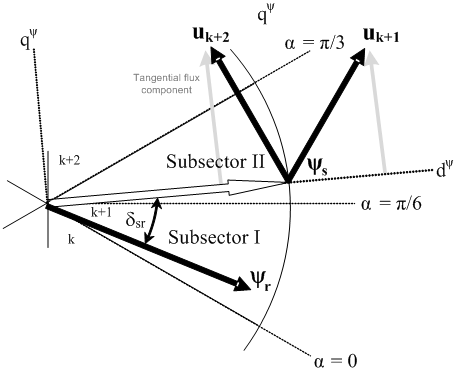
\includegraphics[width=7cm]{figure1}
%% make sure to add \vspace{.7em} before figure's caption
\vspace{.7em}
\caption{Effects of selecting different switching under dynamic condition}
\end{figure}

\begin{table}[H]
\centering
\fontsize{8pt}{10pt}\selectfont
\caption{The performance of ...}
\begin{tabular}{ccc}
\hline
Variable & Speed (rpm) & Power (kW) \\
\hline
x & 10 & 8.6 \\
y & 15 & 12.4 \\
z & 20 & 15.3 \\
\hline
\end{tabular}
\end{table}

\begin{figure}[H]
\centering
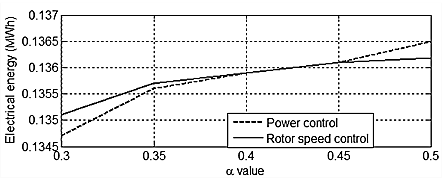
\includegraphics[scale=0.7]{figure2a}\\
(a)\\
\vspace{.7em}
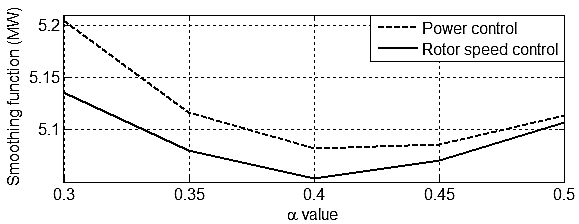
\includegraphics[scale=0.55]{figure2b}\\
(b)\\
	%% make sure to add \vspace{.7em} before figure's caption
\vspace{.7em}
\caption{Comparing simulation results in wind turbine performance with the power control mode to that with the rotor speed control mode in (a) energy output and (b) smoothing function}
\end{figure}

\section{Results and Discussion}
\label{}
This section explains the results of research and at the same time is given the comprehensive discussion. Results can be presented in figures, graphs, tables and others that make the reader understand easily [14], [15]. The discussion can be made in several sub-sections.

\subsection{Sub section 1}
Equations should be placed at the center of the line and provided consecutively with equation numbers in parentheses flushed to the right margin, as in (1). The use of Microsoft Equation Editor or MathType is preferred.

\begin{equation}
E_v - E = \frac{\hbar}{2.m}(k_x^2 + k_y^2)
\end{equation}
%% make sure to add \vspace{.005em} after the end of equation
All symbols that have not been mentioned in the equation should be explained in the following text.


\subsection{Sub section 2}
Proper citation of other works should be made to avoid plagiarism. When referring to a reference item, please use the reference number as in [16] or [17] for multiple references. The use of ”Ref [18]...” should be employed for any reference citation at the beginning of sentence. For any reference with more than 3 or more authors, only the first author is to be written followed by \emph{et al.} (e.g. in [19]). Examples of reference items of different categories shown in the References section. Each item in the references section should be typed using 8 pt font size [20]–[25].

\subsubsection {Subsub section 1}
yy

\subsubsection {Subsub section 2}
zz

\section{Conclusion}
\label{}
Provide a statement that what is expected, as stated in the "INTRODUCTION" section can ultimately result in "RESULTS AND DISCUSSION" section, so there is compatibility. Moreover, the prospects for the development of research results and the application of further studies can also be added to the next (based on the results and discussion).

\section*{ACKNOWLEDGMENTS (if applicable)}
\label{}
This section should acknowledge individuals who provided personal assistance to the work but do not meet the criteria for authorship, detailing their contributions. It is imperative to obtain consent from all individuals listed in the acknowledgments.

\section*{FUNDING INFORMATION (mandatory)}
\label{}
This section should describe sources of funding agency that have supported the work. Authors should state how the research described in their article was funded, including grant numbers if applicable. Include the following (or similar) statement if there is no funding involved: Authors state no funding involved.

\section*{AUTHOR CONTRIBUTIONS STATEMENT (mandatory)}
\label{}
This journal uses the Contributor Roles Taxonomy (CRediT) to recognize individual author contributions, reduce authorship disputes, and facilitate collaboration. \textbf{The recommended number of authors is at least two, with one of them designated as the corresponding author.} The corresponding author will be responsible for all correspondence related to the paper and must ensure that the other authors are included in the communication regarding submission, revision, and publication processes. We encourage authors to include a statement in the paper that shares and accurately describes each author's contribution. \textbf{To be eligible for authorship, each individual must have contributed to at least one of the following: conceptualization, methodology, formal analysis, or investigation, as well as at least one aspect of writing (either original draft preparation or writing reviews and editing).}

\begin{table}[H]
	\centering
	\selectfont
	\begin{tabular}{lcccccccccccccc}
		\hline
		\textbf{Name of Author}\quad\quad\quad\quad\quad\quad\quad & \cellcolor[HTML]{D8F0F8}\textbf{C} & \cellcolor[HTML]{D8F0F8}\textbf{M} & \textbf{So} & \textbf{Va} & \cellcolor[HTML]{D8F0F8}\textbf{Fo} & \cellcolor[HTML]{D8F0F8}\textbf{I} & \textbf{R} & \textbf{D} & \cellcolor[HTML]{FDE9D9}\textbf{O} & \cellcolor[HTML]{FDE9D9}\textbf{E} & \textbf{Vi} & \textbf{Su} & \textbf{P} & \textbf{Fu} \\
		\hline
		Author 1 name & \cellcolor[HTML]{D8F0F8}\checkmark & \cellcolor[HTML]{D8F0F8}\checkmark & \checkmark & \checkmark & \cellcolor[HTML]{D8F0F8}\checkmark & \cellcolor[HTML]{D8F0F8}\checkmark &  & \checkmark & \cellcolor[HTML]{FDE9D9}\checkmark & \cellcolor[HTML]{FDE9D9}\checkmark &  &  & \checkmark &  \\
		Author 2 name &  \cellcolor[HTML]{D8F0F8}& \cellcolor[HTML]{D8F0F8}\checkmark &  &  & \cellcolor[HTML]{D8F0F8} & \cellcolor[HTML]{D8F0F8}\checkmark &  & \checkmark & \cellcolor[HTML]{FDE9D9}\checkmark & \cellcolor[HTML]{FDE9D9}\checkmark & \checkmark & \checkmark &  &  \\
		Author 3 name & \cellcolor[HTML]{D8F0F8}\checkmark & \cellcolor[HTML]{D8F0F8} & \checkmark & \checkmark & \cellcolor[HTML]{D8F0F8} & \cellcolor[HTML]{D8F0F8}\checkmark &  &  & \cellcolor[HTML]{FDE9D9}\checkmark & \cellcolor[HTML]{FDE9D9} & \checkmark &  & \checkmark & \\
		... & \cellcolor[HTML]{D8F0F8} & \cellcolor[HTML]{D8F0F8} &  &  &\cellcolor[HTML]{D8F0F8} & \cellcolor[HTML]{D8F0F8} &  &  & \cellcolor[HTML]{FDE9D9} & \cellcolor[HTML]{FDE9D9} &  &  &  & \\
		Author x name & \cellcolor[HTML]{D8F0F8} & \cellcolor[HTML]{D8F0F8} &  &  & \cellcolor[HTML]{D8F0F8}\checkmark & \cellcolor[HTML]{D8F0F8} &\checkmark &  & \cellcolor[HTML]{FDE9D9} & \cellcolor[HTML]{FDE9D9}\checkmark &  & \checkmark &  & \checkmark\\
		\hline
		\multicolumn{15}{c}{
			\begin{tabular}{llllll}
				&&&&&\\
				C &: 	\textbf{C}\fontsize{8}{10}\selectfont onceptualization \quad\quad\quad\quad\quad\quad& I &: 	\textbf{I}\fontsize{8}{10}\selectfont nvestigation & Vi&: 	\textbf{Vi}\fontsize{8}{10}\selectfont sualization  \\
				M &: 	\textbf{M}\fontsize{8}{10}\selectfont ethodology & R &: 	\textbf{R}\fontsize{8}{10}\selectfont esources & Su&: 	\textbf{Su}\fontsize{8}{10}\selectfont pervision  \\
				So&: 	\textbf{So}\fontsize{8}{10}\selectfont ftware & D &:	\textbf{D}\fontsize{8}{10}\selectfont ata Curation & P &: 	\textbf{P}\fontsize{8}{10}\selectfont roject Administration  \\
				Va&: 	\textbf{Va}\fontsize{8}{10}\selectfont lidation & O &:	\fontsize{8}{10}\selectfont Writing - \fontsize{10}{12}\selectfont \textbf{O}\fontsize{8}{10}\selectfont riginal Draft & Fu&: 	\textbf{Fu}\fontsize{8}{10}\selectfont nding Acquisition \\
				Fo&: 	\textbf{Fo}\fontsize{8}{10}\selectfont rmal Analysis & E &:	\fontsize{8}{10}\selectfont Writing - Review \& \fontsize{10}{12}\selectfont\textbf{E}\fontsize{8}{10}\selectfont diting \quad\quad\quad\quad\quad\quad&  \\
			\end{tabular}
		}
	\end{tabular}
\end{table}



\noindent See the examples below:
\begin{table}[H]
	\centering
	\selectfont
	\begin{tabular}{lcccccccccccccc}
		\hline
		\textbf{Name of Author}\quad\quad\quad\quad\quad & \cellcolor[HTML]{D8F0F8}\textbf{C} & \cellcolor[HTML]{D8F0F8}\textbf{M} & \textbf{So} & \textbf{Va} & \cellcolor[HTML]{D8F0F8}\textbf{Fo} & \cellcolor[HTML]{D8F0F8}\textbf{I} & \textbf{R} & \textbf{D} & \cellcolor[HTML]{FDE9D9}\textbf{O} & \cellcolor[HTML]{FDE9D9}\textbf{E} & \textbf{Vi} & \textbf{Su} & \textbf{P} & \textbf{Fu} \\
		\hline
		Suttichai Premrudeeprechacharn & \cellcolor[HTML]{D8F0F8}\checkmark & \cellcolor[HTML]{D8F0F8}\checkmark & \checkmark & \checkmark & \cellcolor[HTML]{D8F0F8}\checkmark &\cellcolor[HTML]{D8F0F8} \checkmark &  & \checkmark & \cellcolor[HTML]{FDE9D9}\checkmark &\cellcolor[HTML]{FDE9D9} \checkmark &  &  & \checkmark &  \\
		Angela Amphawan & \cellcolor[HTML]{D8F0F8} & \cellcolor[HTML]{D8F0F8}\checkmark &  &  & \cellcolor[HTML]{D8F0F8} & \cellcolor[HTML]{D8F0F8}\checkmark &  & \checkmark &\cellcolor[HTML]{FDE9D9} \checkmark & \cellcolor[HTML]{FDE9D9}\checkmark & \checkmark & \checkmark &  &  \\
		Almoataz Y. Abdelaziz & \cellcolor[HTML]{D8F0F8}\checkmark &\cellcolor[HTML]{D8F0F8}  & \checkmark & \checkmark & \cellcolor[HTML]{D8F0F8} & \cellcolor[HTML]{D8F0F8}\checkmark &  &  & \cellcolor[HTML]{FDE9D9}\checkmark &\cellcolor[HTML]{FDE9D9}  & \checkmark &  & \checkmark & \checkmark\\
		\hline
	\end{tabular}
\end{table}

\section*{CONFLICT OF INTEREST STATEMENT (mandatory)}
\label{}
To ensure fair and objective decision-making, authors must declare any associations that pose a conflict of interest (financial, personal, or professional) in connection with manuscripts. Non-financial competing interests include a declaration of political, personal, religious, ideological, academic, and intellectual competing interests. The authors declare that they have no known competing financial interests or personal relationships that could have appeared to influence the work reported in this paper. If there are no conflicts of interest, please include the following author's statement: Authors state no conflict of interest.

\section*{INFORMED CONSENT (if applicable)}
\label{}
The protection of privacy is a legal right that must not be breached without individual informed consent. In cases where the identification of personal information is necessary for scientific reasons, authors should obtain full documentation of informed consent, including written permission from the patient prior to inclusion in the study. Incorporate the following (or a similar) statement: We have obtained informed consent from all individuals included in this study.

\section*{ETHICAL APPROVAL (if applicable)}
\label{}
When papers talk about using people or animals, authors should make it clear that the research followed all national rules and institutional policies, and it was approved by the authors' institutional review board or a similar committee. The Helsinki Declaration's tenets must guide all investigations involving human subjects. Authors must also identify the committee or review board approving the experiments and provide a statement indicating approval of the research. Incorporate the following (or a similar) statement: The research related to human use has been complied with all the relevant national regulations and institutional policies in accordance with the tenets of the Helsinki Declaration and has been approved by the authors' institutional review board or equivalent committee; or: The research related to animal use has been complied with all the relevant national regulations and institutional policies for the care and use of animals.

\section*{DATA AVAILABILITY (mandatory)}
\label{}
The data availability statement is a valuable link between a paper’s results and the supporting evidence. It is a brief statement about whether the authors of an article have made the evidence supporting their findings available, and if so, where readers may access it. Data availability statements help to promote transparency and reproducibility in research and to increase the visibility of valuable evidence produced or gathered during the course of research. As part of our commitment to supporting open research, our journal now requires all manuscripts to include a data availability statement in order to be accepted for publication. Examples:
\begin{itemize}[topsep=0.3ex, itemsep=0.3ex, parsep=0.2ex]
	\item[-] The supporting data of this study are openly available in [repository's name] at http://doi.org/[doi], reference number [reference number].
	\item[-] The data that support the findings of this study will be available in [repository's name] [URL / DOI link] following a [6 month] embargo from the date of publication to allow for the commercialization of research findings.
	\item[-] The data that support the findings of this study are available on request from the corresponding author, [initials: AB]. The data, which contain information that could compromise the privacy of research participants, are not publicly available due to certain restrictions.
	\item[-] Derived data supporting the findings of this study are available from the corresponding author [initials: AB] on request.
	\item[-] The data that support the findings of this study are available from [third party]. Restrictions apply to the availability of these data, which were used under license for this study. Data are available [from the authors / at URL] with the permission of [third party].
	\item[-] The authors confirm that the data supporting the findings of this study are available within the article [and/or its supplementary materials].
	\item[-] The data that support the findings of this study are available from the corresponding author, [initials: AB], upon reasonable request.
	\item[-] Data availability is not applicable to this paper as no new data were created or analyzed in this study.
\end{itemize}


\section*{REFERENCES}
\label{}
\footnotesize
The main references are international journals and proceedings. All references should be to the most pertinent, up-to-date sources, \textbf{and the minimum number of references} should be \textbf{25} (for original research papers) and \textbf{50} (for review papers). References are written in IEEE style. You can access a more comprehensive guide at http://ipmuonline.com/guide/refstyle.pdf. Use a tool such as EndNote, Mendeley, or Zotero for reference management and formatting; choose \textbf{IEEE style}. Please use a consistent format for references—see examples (8 pt):

\subsection*{[1] Journal/Periodicals}
\footnotesize
\begin{flushleft}
\textsl{Basic Format:\\}
\end{flushleft}
\vspace{-1.1em} 
J. K. Author, “Title of paper,” \textsl{Abbrev. Title of Journal/Periodical}, vol. x, no. x, pp. xx-xx, Abbrev. Month, year, doi: xxx.\\ 
\emph{Examples:}
\begin{enumerate} [leftmargin=*, topsep=0.3ex, itemsep=0.3ex, parsep=0.2ex]
\footnotesize
\item[$-$] M. M. Chiampi and L. L. Zilberti, “Induction of electric field in human bodies moving near MRI: An efficient BEM computational procedure,” \textsl{IEEE Transaction on Biomedical Engineering}, vol. 58, pp. 2787–2793, Oct. 2011, doi: 10.1109/TBME.2011.2158315.
\item[$-$] R. Fardel, M. Nagel, F. Nuesch, T. Lippert, and A. Wokaun, “Fabrication of organic light emitting diode pixels by laser-assisted forward transfer,” \textsl{Appl. Phys. Lett.}, vol. 91, no. 6, Aug. 2007, Art. no. 061103, doi: 10.1063/1.2759475.
\end{enumerate}


\subsection*{[2]	Conference Proceedings}
\footnotesize
\begin{flushleft}
\textsl{Basic Format:\\}
\end{flushleft}
\vspace{-1.1em} 
J. K. Author, “Title of paper,” \textsl{in Abbreviated Name of Conf.}, (location of conference is optional), year, pp. xxx–xxx, doi: xxx. \\
\emph{Examples:}
\begin{enumerate} [leftmargin=*, topsep=0.3ex, itemsep=0.3ex, parsep=0.2ex]
\footnotesize
\item[$-$] G. Veruggio, “The EURON roboethics roadmap,” in \textsl{Proc. Humanoids ’06: 6th IEEE-RAS Int. Conf. Humanoid Robots}, 2006, pp. 612–617, doi: 10.1109/ICHR.2006.321337. 
\item[$-$]	J. Zhao, G. Sun, G. H. Loh, and Y. Xie, “Energy-efficient GPU design with reconfigurable in-package graphics memory,” in \textsl{Proc. ACM/IEEE Int. Symp. Low Power Electron. Design (ISLPED)}, Jul. 2012, pp. 403–408, doi: 10.1145/2333660.2333752.
\end{enumerate}


\subsection*{[3] Book}
\footnotesize
\begin{flushleft}
\textsl{Basic Format:\\}
\end{flushleft}
\vspace{-1.1em} 
\footnotesize
J. K. Author, “Title of chapter in the book,” in \textsl{Title of His Published Book}, X. Editor, Ed., xth ed. City of Publisher, State (only U.S.), Country: Abbrev. of Publisher, year, ch. x, sec. x, pp. xxx–xxx. \\
\textsl{Examples:}
\begin{enumerate} [leftmargin=*, topsep=0.3ex, itemsep=0.3ex, parsep=0.2ex]
\footnotesize
    \item[$-$] A. Taflove, \textsl{Computational Electrodynamics: The Finite-Difference Time-Domain Method} in Computational Electrodynamics II, vol. 3, 2nd ed. Norwood, MA, USA: Artech House, 1996. 
		\item[$-$] R. L. Myer, “Parametric oscillators and nonlinear materials,” in \textsl{Nonlinear Optics}, vol. 4, P. G. Harper and B. S. Wherret, Eds., San Francisco, CA, USA: Academic, 1977, pp. 47–160.
\end{enumerate}


%% References
%%
%% Following citation commands can be used in the body text:
%% Usage of \cite is as follows:
%%   \cite{key}         ==>>  [#]
%%   \cite[chap. 2]{key} ==>> [#, chap. 2]
%%

%% References with BibTeX database:

\bibliographystyle{IEEEtran}
%\bibliography{<your-bib-database>}
%% Authors are advised to use a BibTeX database file for their reference list.
%% The provided style IEEEtran.bst formats references is generally used.

%% For references without a BibTeX database:

\begin{thebibliography} {99} 
\footnotesize
\itemsep 0pt 


%%The main references are international journals and proceedings. All references should be to the most pertinent, up-to-date sources and the minimum of references are 25. References are written in IEEE style. Please use a consistent format for references – see examples below:

%% \bibitem must have the following form:
%%   \bibitem{key}...
%%

\bibitem{1} M. Sigala, A. Beer, L. Hodgson, and A. O’Connor, \emph{Big Data for Measuring the Impact of Tourism Economic Development Programmes: A Process and Quality Criteria Framework for Using Big Data}. 2019.

\bibitem{2} G. Nguyen et al., “Machine Learning and Deep Learning frameworks and libraries for large-scale data mining: a survey,” \textsl{Artif. Intell. Rev.}, vol. 52, no. 1, pp. 77–124, 2019, doi: 10.1007/s10462-018-09679-z

\bibitem{3} C. Shorten and T. M. Khoshgoftaar, “A survey on Image Data Augmentation for Deep Learning,” \textsl{J. Big Data}, vol. 6, no. 1, 2019, doi: 10.1186/s40537-019-0197-0.

\bibitem{4} R. Vinayakumar, M. Alazab, K. P. Soman, P. Poornachandran, A. Al-Nemrat, and S. Venkatraman, “Deep Learning Approach for Intelligent Intrusion Detection System,” \textsl{IEEE Access}, vol. 7, pp. 41525–41550, 2019, doi: 10.1109/ACCESS.2019.2895334.

\bibitem{5} K. Sivaraman, R. M. V. Krishnan, B. Sundarraj, and S. Sri Gowthem, “Network failure detection and diagnosis by analyzing syslog and SNS data: Applying big data analysis to network operations,” \textsl{Int. J. Innov. Technol. Explor. Eng.}, vol. 8, no. 9 Special Issue 3, pp. 883–887, 2019, doi: 10.35940/ijitee.I3187.0789S319.

\bibitem{6} A. D. Dwivedi, G. Srivastava, S. Dhar, and R. Singh, “A decentralized privacy-preserving healthcare blockchain for IoT,” \textsl{Sensors (Switzerland)}, vol. 19, no. 2, pp. 1–17, 2019, doi: 10.3390/s19020326.

\bibitem{7} F. Al-Turjman, H. Zahmatkesh, and L. Mostarda, “Quantifying uncertainty in internet of medical things and big-data services using intelligence and deep learning,” \textsl{IEEE Access}, vol. 7, pp. 115749–115759, 2019, doi: 10.1109/ACCESS.2019.2931637.

\bibitem{8} S. Kumar and M. Singh, “Big data analytics for healthcare industry: Impact, applications, and tools,” \textsl{Big Data Min. Anal.}, vol. 2, no. 1, pp. 48–57, 2019, doi: 10.26599/BDMA.2018.9020031

\bibitem{9} L. M. Ang, K. P. Seng, G. K. Ijemaru, and A. M. Zungeru, “Deployment of IoV for Smart Cities: Applications, Architecture, and Challenges,” \textsl{IEEE Access}, vol. 7, pp. 6473–6492, 2019, doi: 10.1109/ACCESS.2018.2887076.

\bibitem{10} B. P. L. Lau et al., “A survey of data fusion in smart city applications,” \textsl{Inf. Fusion}, vol. 52, no. January, pp. 357–374, 2019, doi: 10.1016/j.inffus.2019.05.004.

\bibitem{11} Y. Wu et al., “Large scale incremental learning,” \textsl{Proc. IEEE Comput. Soc. Conf. Comput. Vis. Pattern Recognit.}, vol. 2019-June, pp. 374–382, 2019, doi: 10.1109/CVPR.2019.00046.

\bibitem{12} A. Mosavi, S. Shamshirband, E. Salwana, K. wing Chau, and J. H. M. Tah, “Prediction of multi-inputs bubble column reactor using a novel hybrid model of computational fluid dynamics and machine learning,” \textsl{Eng. Appl. Comput. Fluid Mech.}, vol. 13, no. 1, pp. 482–492, 2019, doi: 10.1080/19942060.2019.1613448.

\bibitem{13} V. Palanisamy and R. Thirunavukarasu, “Implications of big data analytics in developing healthcare frameworks – A review,” \textsl{J. King Saud Univ. - Comput. Inf. Sci.}, vol. 31, no. 4, pp. 415–425, 2019, doi: 10.1016/j.jksuci.2017.12.007.

\bibitem{14} J. Sadowski, “When data is capital: Datafication, accumulation, and extraction,” \textsl{Big Data Soc.}, vol. 6, no. 1, pp. 1–12, 2019, doi: 10.1177/2053951718820549.

\bibitem{15} J. R. Saura, B. R. Herraez, and A. Reyes-Menendez, “Comparing a traditional approach for financial brand communication analysis with a big data analytics technique,” \textsl{IEEE Access}, vol. 7, pp. 37100–37108, 2019, doi: 10.1109/ACCESS.2019.2905301.

\bibitem{16} D. Nallaperuma et al., “Online Incremental Machine Learning Platform for Big Data-Driven Smart Traffic Management,” textsl{IEEE Trans. Intell. Transp. Syst.}, vol. 20, no. 12, pp. 4679–4690, 2019, doi: 10.1109/TITS.2019.2924883.

\bibitem{17} S. Schulz, M. Becker, M. R. Groseclose, S. Schadt, and C. Hopf, “Advanced MALDI mass spectrometry imaging in pharmaceutical research and drug development,” \textsl{Curr. Opin. Biotechnol.}, vol. 55, pp. 51–59, 2019, doi: 10.1016/j.copbio.2018.08.003.

\bibitem{18} C. Shang and F. You, “Data Analytics and Machine Learning for Smart Process Manufacturing: Recent Advances and Perspectives in the Big Data Era,” \textsl{Engineering}, vol. 5, no. 6, pp. 1010–1016, 2019, doi: 10.1016/j.eng.2019.01.019.

\bibitem{19} Y. Yu, M. Li, L. Liu, Y. Li, and J. Wang, “Clinical big data and deep learning: Applications, challenges, and future outlooks,” \textsl{Big Data Min. Anal.}, vol. 2, no. 4, pp. 288–305, 2019, doi: 10.26599/BDMA.2019.9020007.

\bibitem{20} M. Huang, W. Liu, T. Wang, H. Song, X. Li, and A. Liu, “A queuing delay utilization scheme for on-path service aggregation in services-oriented computing networks,” \textsl{IEEE Access}, vol. 7, pp. 23816–23833, 2019, doi: 10.1109/ACCESS.2019.2899402.

\bibitem{21} G. Xu, Y. Shi, X. Sun, and W. Shen, “Internet of things in marine environment monitoring: A review,” \textsl{Sensors (Switzerland)}, vol. 19, no. 7, pp. 1–21, 2019, doi: 10.3390/s19071711.

\bibitem{22} M. Aqib, R. Mehmood, A. Alzahrani, I. Katib, A. Albeshri, and S. M. Altowaijri, \textsl{Smarter traffic prediction using big data, in-memory computing, deep learning and gpus}, vol. 19, no. 9. 2019.

\bibitem{23} S. Leonelli and N. Tempini, D\textsl{ata Journeys in the Sciences}. 2020.

\bibitem{24} N. Stylos and J. Zwiegelaar, \textsl{Big Data as a Game Changer: How Does It Shape Business Intelligence Within a Tourism and Hospitality Industry Context?} 2019.

\bibitem{25} Q. Song, H. Ge, J. Caverlee, and X. Hu, “Tensor completion algorithms in big data analytics,” \textsl{arXiv}, vol. 13, no. 1, 2017.

\end{thebibliography}


\section*{BIOGRAPHIES OF AUTHORS} 
\normalsize 
In this section, authors are required to provide their professional biography, which should include their academic background, current position, research interests, and any significant contributions to the current study. Additionally, authors should include links to their professional profiles, such as ORCID iD (mandatory) and, if applicable, Google Scholar, Scopus Author ID, or Web of Science (WoS) ResearcherID. This helps establish the author’s academic identity and enhances the visibility of their research.

\noindent Required Information:
\begin{itemize}[topsep=0.3ex, itemsep=0.3ex, parsep=0.2ex]
	\item[-] Full name: Include the author's full name as it appears in official records. If preferred, authors may use the format consistent with his/her Scopus profile.
	\item[-] Email address for each author: Provide the author's professional email address to facilitate correspondence.
	\item[-] Social media account:
	\begin{itemize}[topsep=0.3ex, itemsep=0.3ex, parsep=0.2ex]
		\item[$\blacksquare$] ORCID iD: This is a mandatory. Each author must include their ORCID iD (https://orcid.org/), which helps link his/her research output to their identity.
		\item[$\blacksquare$] Google Scholar Profile: Include the link to the author's Google Scholar profile. If the author does not have a Google Scholar profile, they may create a new one and include the link.
		\item[$\blacksquare$] Scopus Author ID: If available, include the Scopus Author ID to enhance visibility on Scopus.
		\item[$\blacksquare$] Web of Science (WoS) ResearcherID: Include the Web of Science ResearcherID. If the author does not have a WoS profile, they may create a new one and include the link.
	\end{itemize}
	\item[-] Brief biography: Provide a concise overview of the author's academic background, research interests, notable publications, and contributions to the current paper. This should be no longer than 150 to 200 words.
	\item[-] Professional achievements: If available, mention any important awards, recognition, or research projects the author has been involved in.
	\item[-] Photo Submission: Authors must submit a clear, professional headshot (3x4 cm). The photo should be of high quality, well-lit, and not blurry. Avoid using photos that are overly casual or low resolution.
\end{itemize}


\newpage\noindent Below is an example of how to format the biography section for each author:


\section*{BIOGRAPHIES OF AUTHORS} 
%% make sure to add \vspace{-.7em} before \begin{biography}
\vspace{-.7em} 
\small
\begin{biography}[{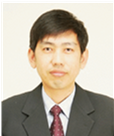
\includegraphics[width=2.5cm,height=4cm,clip,keepaspectratio]{a1}}]
\textbf{Suttichai Premrudeeprechacharn} %% Affiliation and educational background.
\href{https://orcid.org/0000-0001-9902-7729}{
\includegraphics[width=0.02\textwidth]{orcid.png}} 
\href{https://scholar.google.com/citations?user=bwiNxDQAAAAJ}{
\includegraphics[width=0.02\textwidth]{gscholar.png}}
\href{https://www.scopus.com/authid/detail.uri?authorId=6508110941}{
\includegraphics[width=0.02\textwidth]{scopus.png}}
\href{https://publons.com/researcher/3133629/suttichai-premrudeepreechacharn/}{
\includegraphics[width=0.02\textwidth]{wos.png}} received the B.Eng. degree in electrical engineering from Chiang Mai University, Thailand, in 1988 and the M.S. and Ph.D. degrees in electric power engineering from Rensselaer Polytechnic Institute, Troy, NY, in 1992 and 1997, respectively. Currently, he is an Associate Professor at the Department of Electrical Engineering, Chiang Mai University. His research interests include renewable energy, power quality, high quality utility interface, power electronics, power generation, power grids, power supply quality, power transmission reliability, relay protection, power system stability, power transmission lines, power transmission planning, power transmission protection, battery chargers, circuit breakers, harmonic distortion, hydroelectric power stations, load flow control, overcurrent protection, particle swarm optimisation, power distribution protection, and artificial intelligence applied power system. He can be contacted at email: suttichai@mail.com.
\end{biography}

\begin{biography}[{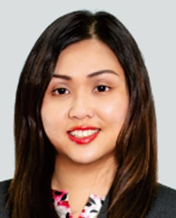
\includegraphics[width=2.5cm,height=4cm,clip,keepaspectratio]{a2}}]
\textbf{Angela Amphawan} %% Affiliation and educational background.
\href{https://orcid.org/0000-0003-2838-8679}{
\includegraphics[width=0.02\textwidth]{orcid.png}} 
\href{https://scholar.google.com/citations?user=kdOwHMIAAAAJ&hl=en&oi=sra}{
\includegraphics[width=0.02\textwidth]{gscholar.png}}
\href{https://www.scopus.com/authid/detail.uri?authorId=35730929200}{
\includegraphics[width=0.02\textwidth]{scopus.png}}
\href{https://publons.com/researcher/1170442/dr-angela-amphawan/}{
\includegraphics[width=0.02\textwidth]{wos.png}} holds a PhD in optical communications from University of Oxford, United Kingdom. She is currently Head of the Optical Technology Group at the Universiti Utara Malaysia. She is also a Fulbright Fellow at Massachusetts Institute of Technology (MIT), Cambridge, USA. The pervasiveness of the Internet in today’s digital society brings to light her work on digital convergence for media communications, focusing on optical fiber communications, free-space optics and microwave photonics. Her research has been funded by the Fulbright Foundation, Telekom Malaysia and the Malaysian Ministry of Higher Education. She has been elected on the Scientific Committee and Editorial Review Board for the World Academy of Science, Engineering and Technology. She is also a research affiliate for the Asia Pacific International Telecommunications Union (ITU) and serves on the Editorial Board for the International Journal of Electrical and Computer Engineering as well as the International Journal of Informatics and Communication Technology. In addition, she is a reviewer for leading optical journals such as Optics Express, Optics Letters, Journal of Lightwave Technology and IEEE Photonics Journal. She can be contacted at email: angela@uum.edu.my.
\end{biography}

\begin{biography}[{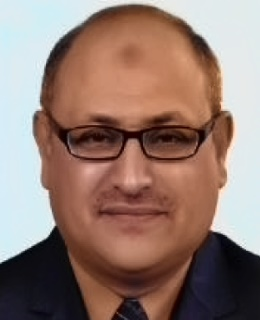
\includegraphics[width=2.5cm,height=4cm,clip,keepaspectratio]{a3}}]
\textbf{Almoataz Y. Abdelaziz} %% Affiliation and educational background.
\href{https://orcid.org/0000-0001-5903-5257}{
\includegraphics[width=0.02\textwidth]{orcid.png}} 
\href{https://scholar.google.com/citations?hl=en&user=646RieYAAAAJ}{
\includegraphics[width=0.02\textwidth]{gscholar.png}}
\href{https://www.scopus.com/authid/detail.uri?authorId=7003870872}{
\includegraphics[width=0.02\textwidth]{scopus.png}}
\href{https://publons.com/researcher/2894894/almoataz-y-abdelaziz/}{
\includegraphics[width=0.02\textwidth]{wos.png}} received the B.Sc. and M.Sc. degrees in electrical engineering from Ain Shams University, Cairo, Egypt, in 1985 and 1990, respectively, and the Ph.D. degree in electrical engineering according to the channel system between Ain Shams University, Egypt, and Brunel University, U.K., in 1996. He has been a professor of electrical power engineering with Ain Shams University, since 2007. He is currently the Vice Dean of Faculty of Engineering and Technology, Future University in Egypt, Cairo, Egypt. He has authored or coauthored more than 400 refereed journal and conference papers, 25 book chapters, and three edited books with Elsevier and Springer. His research interests include the applications of artificial intelligence, evolutionary and heuristic optimization techniques to power system planning, operation, and control. He can be contacted at email: almoataz@mail.com.
\end{biography}

\end{document}

%%
%% End of file `iaesarticle.tex'. 